\documentclass{ximera}


\graphicspath{
  {./}
  {ximeraTutorial/}
  {basicPhilosophy/}
}

\newcommand{\mooculus}{\textsf{\textbf{MOOC}\textnormal{\textsf{ULUS}}}}

\usepackage{tkz-euclide}\usepackage{tikz}
\usepackage{tikz-cd}
\usetikzlibrary{arrows}
\tikzset{>=stealth,commutative diagrams/.cd,
  arrow style=tikz,diagrams={>=stealth}} %% cool arrow head
\tikzset{shorten <>/.style={ shorten >=#1, shorten <=#1 } } %% allows shorter vectors

\usetikzlibrary{backgrounds} %% for boxes around graphs
\usetikzlibrary{shapes,positioning}  %% Clouds and stars
\usetikzlibrary{matrix} %% for matrix
\usepgfplotslibrary{polar} %% for polar plots
\usepgfplotslibrary{fillbetween} %% to shade area between curves in TikZ
\usetkzobj{all}
\usepackage[makeroom]{cancel} %% for strike outs
%\usepackage{mathtools} %% for pretty underbrace % Breaks Ximera
%\usepackage{multicol}
\usepackage{pgffor} %% required for integral for loops



%% http://tex.stackexchange.com/questions/66490/drawing-a-tikz-arc-specifying-the-center
%% Draws beach ball
\tikzset{pics/carc/.style args={#1:#2:#3}{code={\draw[pic actions] (#1:#3) arc(#1:#2:#3);}}}



\usepackage{array}
\setlength{\extrarowheight}{+.1cm}
\newdimen\digitwidth
\settowidth\digitwidth{9}
\def\divrule#1#2{
\noalign{\moveright#1\digitwidth
\vbox{\hrule width#2\digitwidth}}}






\DeclareMathOperator{\arccot}{arccot}
\DeclareMathOperator{\arcsec}{arcsec}
\DeclareMathOperator{\arccsc}{arccsc}

















%%This is to help with formatting on future title pages.
\newenvironment{sectionOutcomes}{}{}


\title{Graph Symbols}

\begin{document}

\begin{abstract}
communication
\end{abstract}
\maketitle



We can easily define a function via a graph.  However, it is not so easy to decipher exact information from a graph, especially when the curve is drawn by hand.  Therefore, in addition to the points on the curve, we include other symbols to help people read the graph and understand the function.  These are communication symbols.  They help the reader understand what is drawn and what is not drawn.  This is the beginning of our attention to \textbf{\textcolor{purple!85!blue}{rigor}}.



\section{Rigor}

$\blacktriangleright$ \textbf{\textcolor{purple!85!blue}{What is Rigor in a Mathematics Classroom?}} \\


\begin{quote}
\textbf{\textcolor{purple!85!blue}{Rigor}} is when students use mathematical language to communicate effectively and to describe their reasoning with clarity and precision.  Students make understood ``How do we know we have accounted for everything?''
\end{quote}



\textbf{\textcolor{blue!55!black}{Rigor}} is one of the main threads in this course along with function structure.  It will take a lot of communication back and forth to learn how to present \textbf{\textcolor{purple!85!blue}{rigorous}} explanations. \\


We have already commented that graphs are inherently inaccurate, so they might seem an odd place to introduce \textbf{\textcolor{purple!85!blue}{rigor}}.  On the other hand, we have noted that graphs are communcation tools. This makes them an easy entrance to the ideas of \textbf{\textcolor{purple!85!blue}{rigor}}.  We can begin by using auxillary graph symbols to clarify our graphical communication. Their presence and absence communicate information about the function.










\section{Endpoints}


Points are dimensionless objects.  They are too small to actually see.  When we draw a graph, the thickness of the pencil or pen is already an exaggeration of the underlying points and makes the endpoints a mystery.  How would you tell if the very last point of a curve was included or not? Therefore, we exaggerate even more for the endpoints, so that the reader immediately understands whether or not they are plotted.

We use big solid dots (blobs, discs) to illustrate an endpoint is a part of the drawing. We use big hollow dots (circles) when the actual last point is not included. 


In the graph on the left, it is difficult to tell if the endpoints are included or not.  The graph on the right makes this clear.

\begin{image}
\begin{tikzpicture}
    \begin{axis}[name = without,
            	domain=-5:5, ymax=5, xmax=5, ymin=-5, xmin=-5,
            	axis lines =center, xlabel=$x$, ylabel=$y$,
            	every axis y label/.style={at=(current axis.above origin),anchor=south},
            	every axis x label/.style={at=(current axis.right of origin),anchor=west},
            	axis on top,
          		]

        \addplot [draw=penColor, very thick, smooth, domain=(-3:4)] {0.5*x-1};
    \end{axis}





     \begin{axis}[
            	at={(without.outer east)}, anchor=outer west, domain=-5:5, ymax=5, xmax=5, ymin=-5, xmin=-5,
            	axis lines =center, xlabel=$x$, ylabel=$y$,
            	every axis y label/.style={at=(current axis.above origin),anchor=south},
            	every axis x label/.style={at=(current axis.right of origin),anchor=west},
            	axis on top,
          		]

        \addplot [draw=penColor, very thick, smooth, domain=(-3:4)] {0.5*x-1};
        \addplot[color=penColor,fill=penColor,only marks,mark=*] coordinates{(-3, -2.5)};
        \addplot[color=penColor,fill=white,only marks,mark=*] coordinates{(4, 1)};
    \end{axis}



\end{tikzpicture}
\end{image}


The big exaggerated dots are just for the single endpoints.  The curve on the right does not actually include a circle as part of the curve. That circle is an exaggerated single hollow dot indicating that the point $(4, 1)$ is not part of the curve.







\section{Arrows}


When we use graphs to define functions, we need to communicate the domain. This is difficult when the domain is large, such as $(-\infty, \infty)$. The paper we draw on is only inches wide.  So, we include several additional graph symbols to help the reader understand what is happening out of view.

Arrows at the ends of curves signal that the curve continues its current pattern.


In the graph on the left, it is difficult to decide if the domain is the interval $(-3, 4)$ or not.  The graph on the right makes this clear.

\begin{image}
\begin{tikzpicture}
    \begin{axis}[name = without,
            	domain=-5:5, ymax=5, xmax=5, ymin=-5, xmin=-5,
            	axis lines =center, xlabel=$x$, ylabel=$y$,
            	every axis y label/.style={at=(current axis.above origin),anchor=south},
            	every axis x label/.style={at=(current axis.right of origin),anchor=west},
            	axis on top,
          		]

        \addplot [draw=penColor, very thick, smooth, domain=(-3:4)] {0.5*x-1};

    \end{axis}





     \begin{axis}[
            	at={(without.outer east)}, anchor=outer west, domain=-5:5, ymax=5, xmax=5, ymin=-5, xmin=-5,
            	axis lines =center, xlabel=$x$, ylabel=$y$,
            	every axis y label/.style={at=(current axis.above origin),anchor=south},
            	every axis x label/.style={at=(current axis.right of origin),anchor=west},
            	axis on top,
          		]

        \addplot [draw=penColor, very thick, smooth, domain=(-3:4), ->] {0.5*x-1};
        \addplot[color=penColor,only marks,mark=*] coordinates{(-3,-2.5)}; 

    \end{axis}



\end{tikzpicture}
\end{image}


Here, the arrow tells the reader that the curve continues its current linear pattern indefinitely to the right.  The domain is $[-3, \infty)$.











\section{Asymptotes}


Arrows at the ends of curves signal that the curve continues with its current pattern. However, this may not not be enough.  Many functions have curves that continue moving down and to the right, however, their movement has a boundary. We use dashed lines to indicate that a curve is approaching this line pattern.


\begin{image}
\begin{tikzpicture}
     \begin{axis}[
            	domain=-10:10, ymax=10, xmax=10, ymin=-10, xmin=-10,
            	axis lines =center, xlabel=$x$, ylabel=$y$,
                 ytick={-10,-8,-6,-4,-2,2,4,6,8,10},
            xtick={-10,-8,-6,-4,-2,2,4,6,8,10},
            yticklabels={$-10$,$-8$,$-6$,$-4$,$-2$,$2$,$4$,$6$,$8$,$10$}, 
            xticklabels={$-10$,$-8$,$-6$,$-4$,$-2$,$2$,$4$,$6$,$8$,$10$},
            ticklabel style={font=\scriptsize},
            	every axis y label/.style={at=(current axis.above origin),anchor=south},
            	every axis x label/.style={at=(current axis.right of origin),anchor=west},
            	axis on top,
          		]

        
        \addplot [draw=penColor, very thick, smooth, domain=(-6:3), <->] {1/(x-3) + 2};
        \addplot [draw=penColor, very thick, smooth, domain=(3:8), <->] {1/(x-3) + 2};

        \addplot [line width=0.5, gray, dashed,samples=100,domain=(-9:9)] ({3},{x});
        \addplot [line width=0.5, gray, dashed,samples=100,domain=(-9:9)] ({x},{2});


    \end{axis}



\end{tikzpicture}
\end{image}


The arrows tell the reader that the curve continues its current pattern, for example the right piece of the curve continues to move up and to the left.  The dashed vertical asymptote tells us that the leftward movement does not go past the line $x=3$.  The curve continues to go up indefinitely while getting closer and closer to the asymptote, without hitting the asymptote. 

This tells us that the function becomes unbounded as you get closer to $3$ in the domain. \\




Horizontal asymptotes give similar information.  The function graphed below gets closer to the value of $2$ as the values of the domain get bigger.   Unlike with vertical asymptotes, the graph of a function can oscillate back-and-forth across a horizontal asymptote.




\begin{image}
\begin{tikzpicture}
     \begin{axis}[
                domain=-10:10, ymax=10, xmax=10, ymin=-10, xmin=-10,
                axis lines =center, xlabel=$x$, ylabel=${y=f(x)}$,
                ytick={-10,-8,-6,-4,-2,2,4,6,8,10},
                xtick={-10,-8,-6,-4,-2,2,4,6,8,10},
                yticklabels={$-10$,$-8$,$-6$,$-4$,$-2$,$2$,$4$,$6$,$8$,$10$}, 
                xticklabels={$-10$,$-8$,$-6$,$-4$,$-2$,$2$,$4$,$6$,$8$,$10$},
                ticklabel style={font=\scriptsize},
                every axis y label/.style={at=(current axis.above origin),anchor=south},
                every axis x label/.style={at=(current axis.right of origin),anchor=west},
                axis on top,
                ]

        
        \addplot [draw=penColor, very thick, smooth, domain=(-6:10), <->] {10*sin(deg(x))/((x+10)^1.2) + e^(-x-5) + 2};
        %\addplot [draw=penColor, very thick, smooth, domain=(3:8), <->] {1/(x-3) + 2};

        %\addplot [line width=1, gray, dashed,samples=100,domain=(-9:9)] ({3},{x});
        \addplot [line width=0.5, gray, dashed,samples=100,domain=(1:9)] ({x},{2});


    \end{axis}



\end{tikzpicture}
\end{image}


The values of the function, $f(x)$, get closer (or approach) $2$ as we move through the domain, heading to infinity.  \\

And, of course, we have algebraic notation to communicate this thought.


\[
\lim_{x \to \infty} f(x) = 2
\]


This ``limit notation'' is our algebraic way of communicating that the function $f(x)$ approaches the value $2$ as the domain values become unbounded positively.  More on limit notation later in the course.







\section{Ellipsis}


Sometimes an arrow at the end of the curve may give the wrong impression.  






\begin{image}
\begin{tikzpicture}
    \begin{axis}[
            domain=-10:10, ymax=2, xmax=10, ymin=-2, xmin=-10,
            axis lines =center, xlabel=$t$, ylabel=$y$,
            ytick={-2,-1,1,2},
            xtick={-10,-8,-6,-4,-2,2,4,6,8,10},
            yticklabels={$-2$,$-1$,$1$,$2$}, 
            xticklabels={$-10$,$-8$,$-6$,$-4$,$-2$,$2$,$4$,$6$,$8$,$10$},
            ticklabel style={font=\scriptsize},
            every axis y label/.style={at=(current axis.above origin),anchor=south},
            every axis x label/.style={at=(current axis.right of origin),anchor=west},
            axis on top
          ]
          
    \addplot [draw=penColor,very thick,smooth,domain=(-2:-1)] {x+2};
    \addplot [draw=penColor,very thick,smooth,domain=(-1:0)] {-x};

    \addplot [draw=penColor,very thick,smooth,domain=(0:1)] {x};
    \addplot [draw=penColor,very thick,smooth,domain=(1:2)] {-x+2};

    \addplot [draw=penColor,very thick,smooth,domain=(2:3)] {x-2};
    \addplot [draw=penColor,very thick,smooth,domain=(3:4), ->] {-x+4};






    \end{axis}
\end{tikzpicture}
\end{image}
Just an arrow may be interpretted as the line continuing down.




If the pattern involves some kind of repeated (periodic) shape, then ellipses may be used.



\begin{image}
\begin{tikzpicture}
	\begin{axis}[
            domain=-10:10, ymax=3, xmax=10, ymin=-2, xmin=-10,
            axis lines =center, xlabel=$t$, ylabel=$y$,
            ytick={-2,-1,1,2},
            xtick={-10,-8,-6,-4,-2,2,4,6,8,10},
            yticklabels={$-2$,$-1$,$1$,$2$}, 
            xticklabels={$-10$,$-8$,$-6$,$-4$,$-2$,$2$,$4$,$6$,$8$,$10$},
            ticklabel style={font=\scriptsize},
            every axis y label/.style={at=(current axis.above origin),anchor=south},
            every axis x label/.style={at=(current axis.right of origin),anchor=west},
            axis on top
          ]
          
	\addplot [draw=penColor,very thick,smooth,domain=(-2:-1)] {x+2};
	\addplot [draw=penColor,very thick,smooth,domain=(-1:0)] {-x};

	\addplot [draw=penColor,very thick,smooth,domain=(0:1)] {x};
	\addplot [draw=penColor,very thick,smooth,domain=(1:2)] {-x+2};

	\addplot [draw=penColor,very thick,smooth,domain=(2:3)] {x-2};
	\addplot [draw=penColor,very thick,smooth,domain=(3:4)] {-x+4};



	\addplot[color=penColor,only marks,mark=*] coordinates{(-3,0.5)}; 
	\addplot[color=penColor,only marks,mark=*] coordinates{(-4,0.5)}; 
	\addplot[color=penColor,only marks,mark=*] coordinates{(-5,0.5)}; 

	\addplot[color=penColor,only marks,mark=*] coordinates{(5,0.5)}; 
	\addplot[color=penColor,only marks,mark=*] coordinates{(6,0.5)}; 
	\addplot[color=penColor,only marks,mark=*] coordinates{(7,0.5)}; 




    \end{axis}
\end{tikzpicture}
\end{image}





A graph is a communication tool. We already know that the accuracy has limitations. There are also other limitations that we must deal with.  To that end, a nice graph displays other symbols besides just the points.  These other graphical features help the reader understand the thoughts of the drawer. \\




\begin{warning}
These graphical enhancements are not optional.  They are a requirement of our desire to be \textbf{\textcolor{purple!85!blue}{rigorous}}.
\end{warning}



\begin{question} Reading Graphs

\begin{image}
\begin{tikzpicture}
     \begin{axis}[
            	domain=-10:10, ymax=10, xmax=10, ymin=-10, xmin=-10,
            	axis lines =center, xlabel=$x$, ylabel=$y$,
                ytick={-10,-8,-6,-4,-2,2,4,6,8,10},
                xtick={-10,-8,-6,-4,-2,2,4,6,8,10},
                yticklabels={$-10$,$-8$,$-6$,$-4$,$-2$,$2$,$4$,$6$,$8$,$10$}, 
                xticklabels={$-10$,$-8$,$-6$,$-4$,$-2$,$2$,$4$,$6$,$8$,$10$},
                ticklabel style={font=\scriptsize},
            	every axis y label/.style={at=(current axis.above origin),anchor=south},
            	every axis x label/.style={at=(current axis.right of origin),anchor=west},
            	axis on top,
          		]

        
        \addplot [draw=penColor, very thick, smooth, domain=(-6:3), <->] {1/(x-3) + 2};
        \addplot [draw=penColor, very thick, smooth, domain=(3:8)] {1/(x-3) + 2};

        \addplot [line width=0.5, gray, dashed,samples=100,domain=(-9:9)] ({3},{x});
        \addplot [line width=0.5, gray, dashed,samples=100,domain=(-9:9)] ({x},{2});

        \addplot[color=penColor,only marks,mark=*] coordinates{(3.2,7)}; 
        \addplot[color=penColor,only marks,mark=*] coordinates{(8,2.2)}; 


    \end{axis}



\end{tikzpicture}
\end{image}

\begin{itemize}
\item The graph above has points with $y$-coordinates greater than $5,000$.
\begin{multipleChoice}
\choice {True}
\choice [correct]{False}
\end{multipleChoice} 


\item The graph above has points with $y$-coordinates less than $-5,000$.
\begin{multipleChoice}
\choice [correct]{True}
\choice {False}
\end{multipleChoice}



\item The graph above has points with $x$-coordinates greater than $5,000$.
\begin{multipleChoice}
\choice {True}
\choice [correct]{False}
\end{multipleChoice}



\item The graph above has points with $x$-coordinates less than $-5,000$.
\begin{multipleChoice}
\choice [correct]{True}
\choice {False}
\end{multipleChoice}
\end{itemize}

\end{question}











\section{Missing Symbols}

All of these graphical symbols help the reader understand the graph.  When the symbols are not drawn, then we know the author of the graph does not want us to interpret the graph in that way.


\begin{itemize}
\item If there is no horizontal asymptote, then we should not read that the graph is leveling off and becoming horizontal.
\item If there are no ellipses, then we should not assume the pattern repeats.
\item If there is no arrow, then we should not assume the pattern continues.
\item If there are no solid or hollow endpoints, then we need to question the drawer.
\end{itemize}



The auxillary pieces drawn on a graph give us information and their absence gives us information as well.









\section{Technology}

We are humans communicating to other humans, which is why we take care to create readable and informative graphs. Technology does not have this desire.





\begin{image}
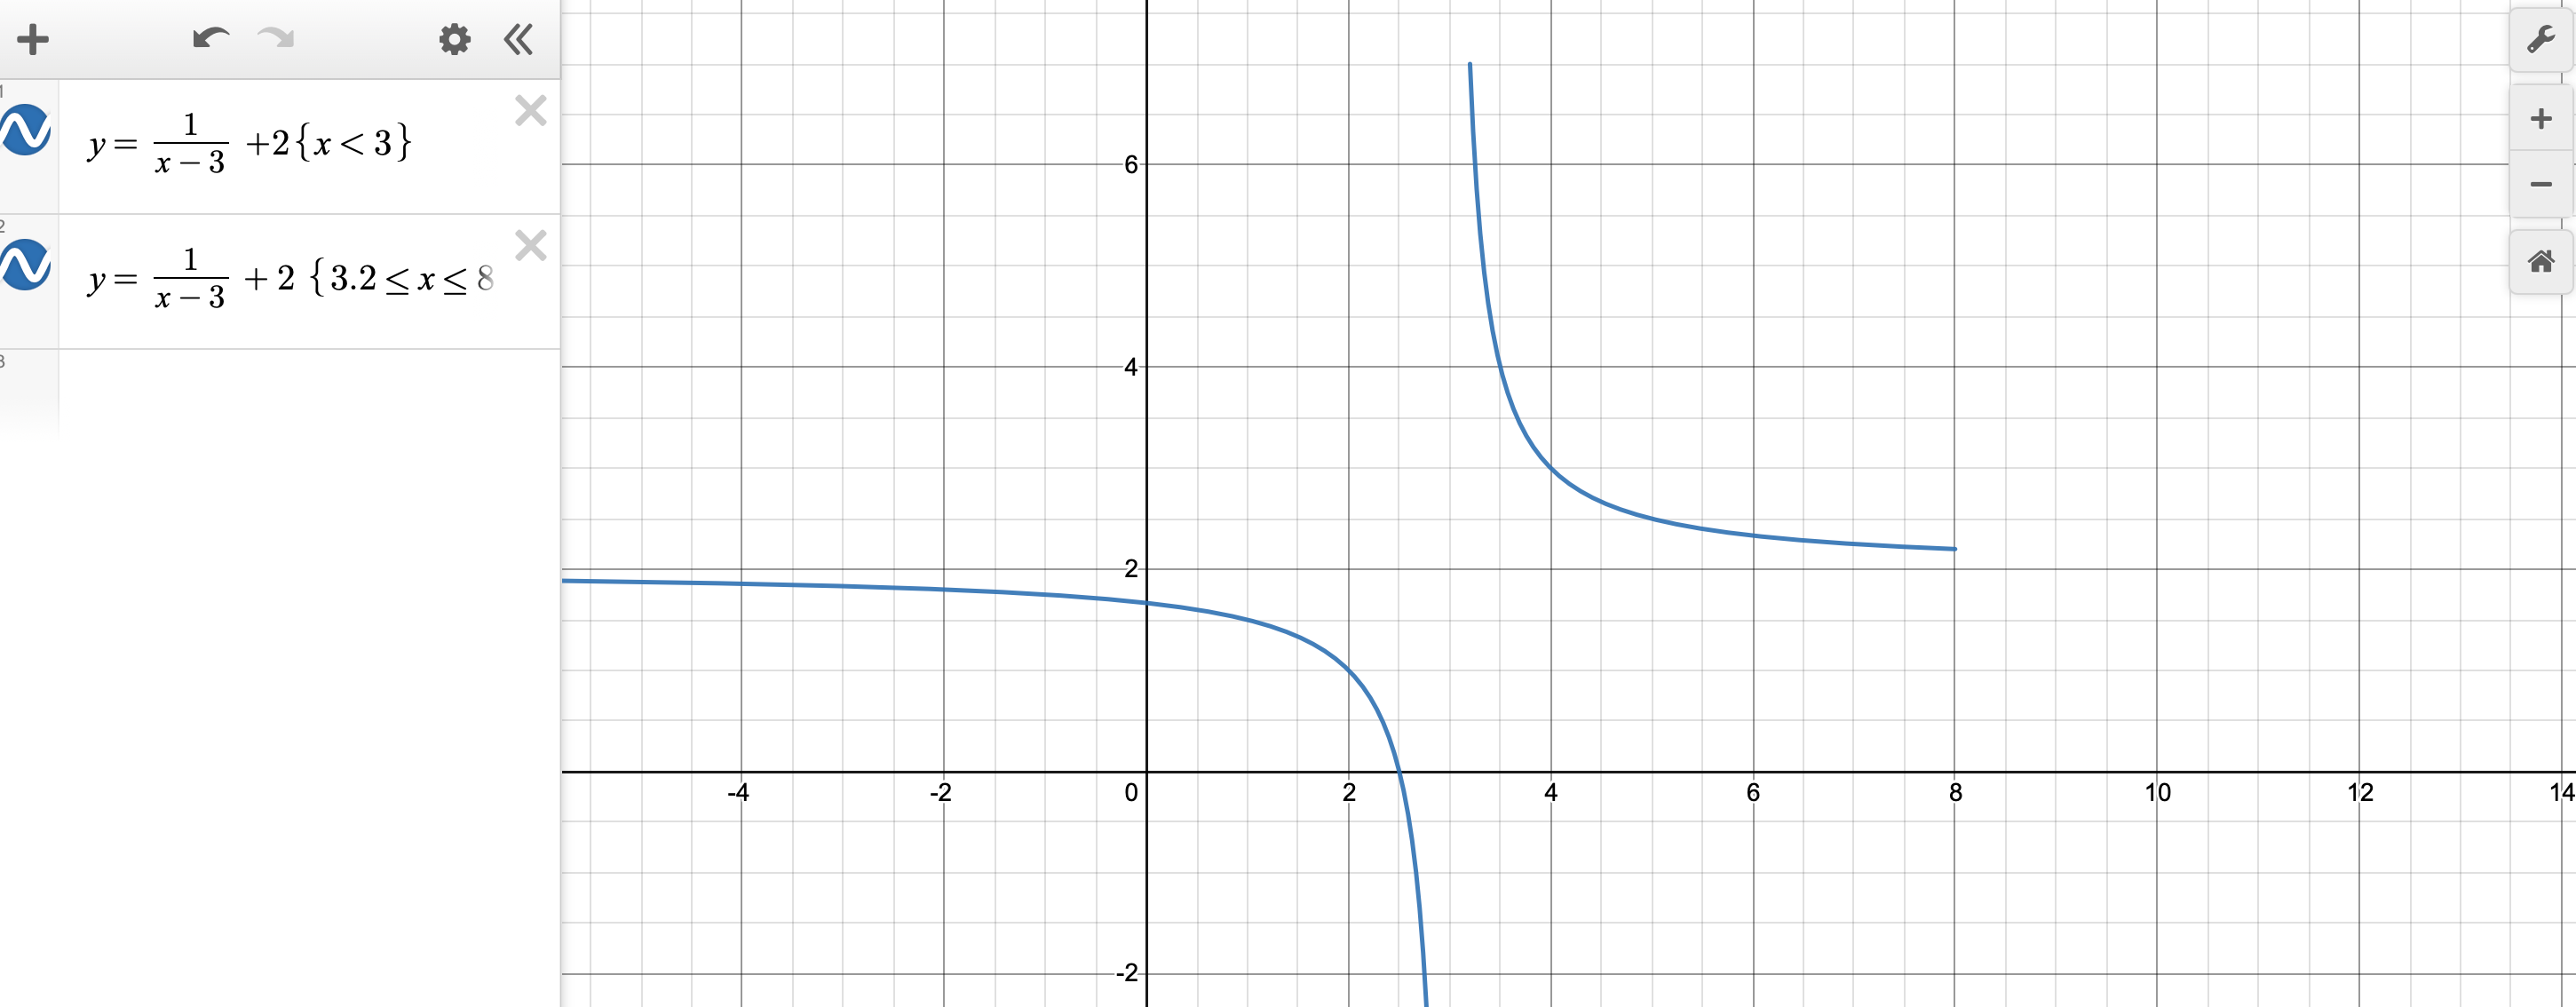
\includegraphics{pics/graph_symbols.png}
\end{image}



When working with technology, we have to accept that it is a machine giving us what it is programmed to give.  We must interpret correctly. \\


When we make our own graphs, then we can hold ourselves to a higher standard.















\begin{center}
\textbf{\textcolor{green!50!black}{ooooo=-=-=-=-=-=-=-=-=-=-=-=-=ooOoo=-=-=-=-=-=-=-=-=-=-=-=-=ooooo}} \\

more examples can be found by following this link\\ \link[More Examples of Graphical Communication]{https://ximera.osu.edu/csccmathematics/precalculus1/precalculus1/graphicalCommunication/examples/exampleList}

\end{center}







\end{document}
